\documentclass[10pt]{article}
\usepackage{amsmath,amssymb}
\usepackage[margin=1in]{geometry}
\usepackage{graphicx}
\usepackage{siunitx}
\begin{document}

\section*{1}

\subsection*{a}

$$V = V_1 + V_2 \Rightarrow I \cdot R_1 = V_1, I \cdot R_2 = V_2$$

$$\hookrightarrow V = I \cdot R_1 + I \cdot R_2 = I(R_1 + R_2)$$

$$\Rightarrow I = \frac{V}{R_1 + R_2}$$


\subsection*{b}

$$R_{eq} = R_1 + R_2 = 1.5 k\Omega = 1500 \Omega$$

$$V_{eq_1} = I \cdot R_1 \Rightarrow I = \frac{V}{R_{eq}} = \frac{9}{1500} A$$

$$V_{eq_1} = \frac{9}{1500} \cdot 500 = 9 \cdot \frac{1}{3} = 3V$$

$$V_{eq_2} = \frac{9}{1500} \cdot 1000 = 9 \cdot \frac{2}{3} = 6V$$

\section*{2}


\begin{center}
	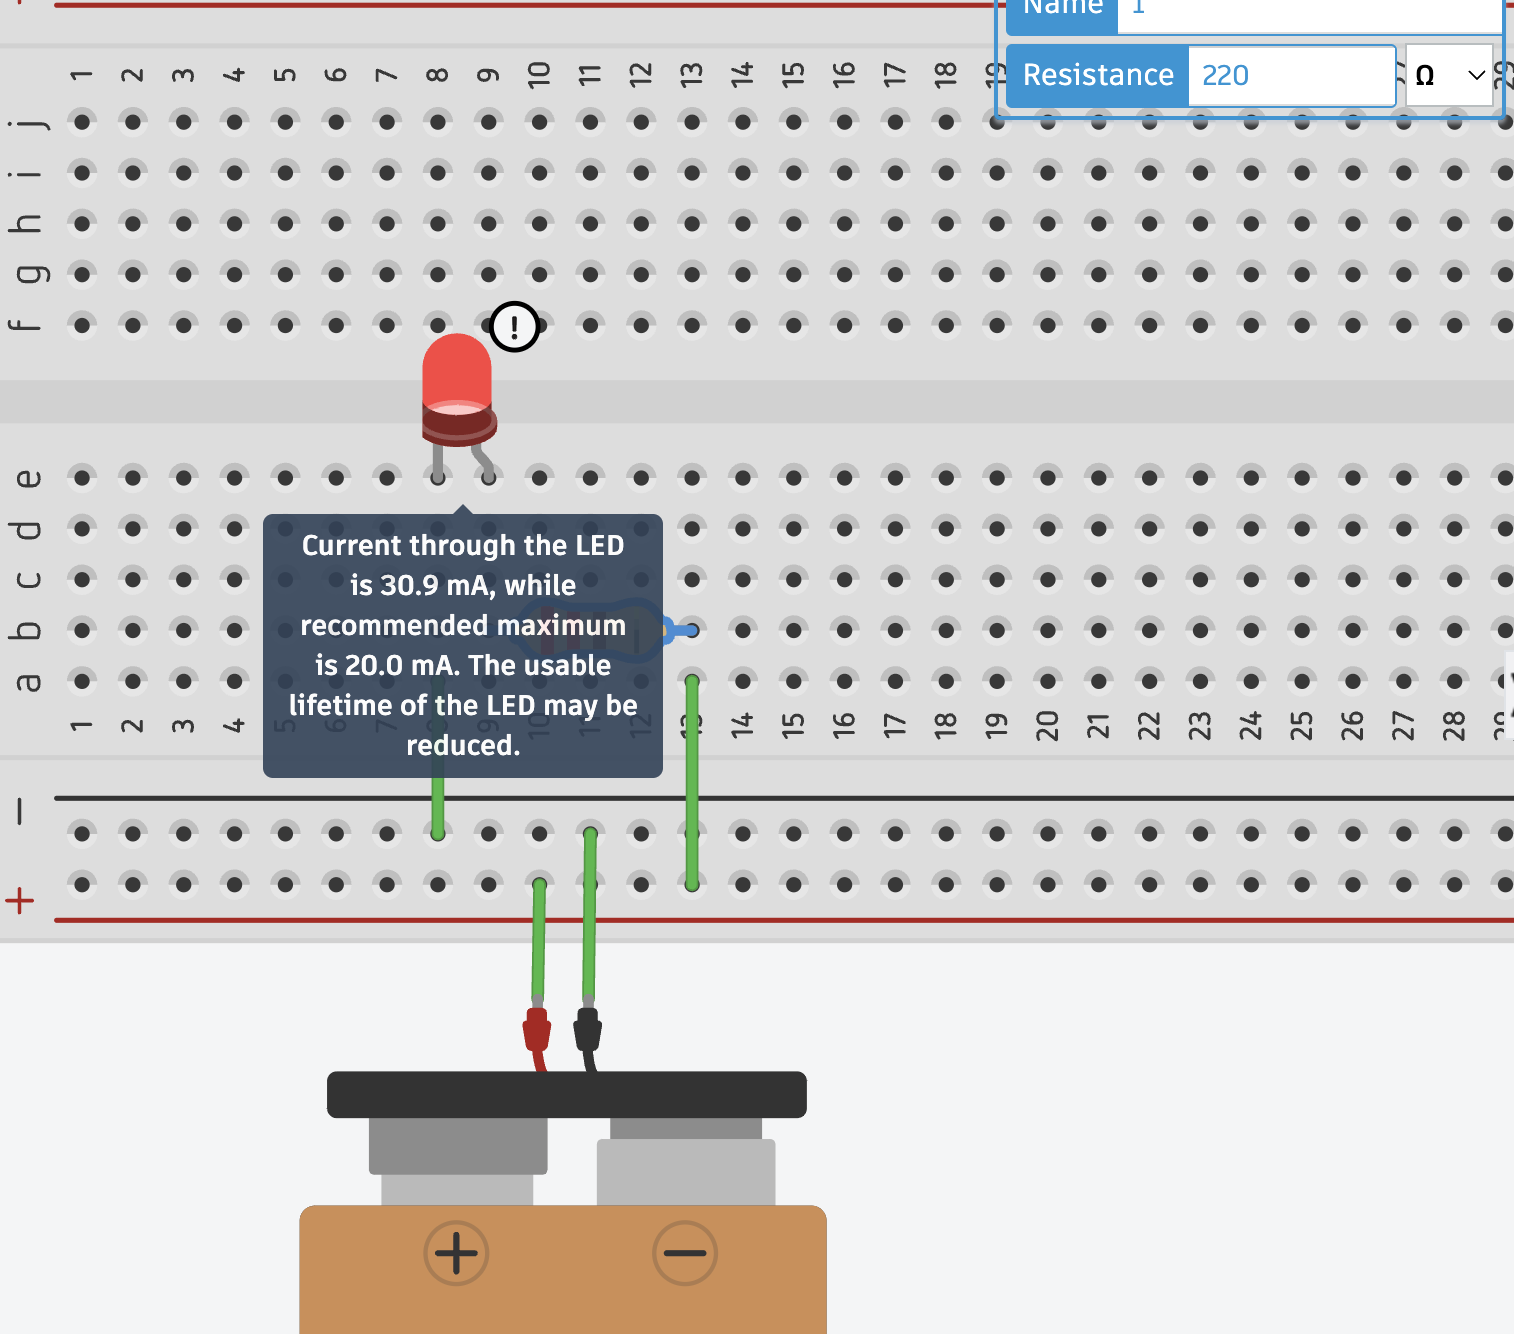
\includegraphics[width=0.5\textwidth]{ledbad.png}
\end{center}

Using KVL:

\[
	9V - 2V - IR = 0 \quad \Rightarrow \quad I = \frac{7V}{R}
\]

\begin{itemize}
	\item Smaller $R$ $\Rightarrow$ Larger $I$ $\Rightarrow$ Brighter LED
	\item But $I > 20$mA may damage the LED
\end{itemize}

\section*{3}

Using Ohm's Law for each branch:
\begin{align*} I_1 &= \frac{V}{R_1} = \frac{9 \, \text{V}}{900 \, \Omega} = 0.01 \, \text{A} \\ I_2 &= \frac{V}{R_2} = \frac{9 \, \text{V}}{450 \, \Omega} = 0.02 \, \text{A} \\ I_3 &= \frac{V}{R_3} = \frac{9 \, \text{V}}{450 \, \Omega} = 0.02 \, \text{A} \end{align*}

\section*{4}
\[
	\frac{1}{R_{eq}} = \frac{R_2 R_3 + R_1 R_3 + R_1 R_2}{R_1 R_2 R_3}
\]
\[
	R_{eq} = \frac{R_1 R_2 R_3}{R_1 R_2 + R_1 R_3 + R_2 R_3}
\]
\[
	\frac{1}{R_{eq}} = \frac{1}{\SI{900}{\ohm}} + \frac{1}{\SI{450}{\ohm}} + \frac{1}{\SI{450}{\ohm}}
\]
\[
	\frac{1}{R_{eq}} = \frac{1}{\SI{900}{\ohm}} + \frac{2}{\SI{900}{\ohm}} + \frac{2}{\SI{900}{\ohm}}
\]
\[
	\frac{1}{R_{eq}} = \frac{1+2+2}{\SI{900}{\ohm}} = \frac{5}{\SI{900}{\ohm}}
\]
\[
	R_{eq} = \frac{\SI{900}{\ohm}}{5} = \SI{180}{\ohm}
\]

\section*{5}

\begin{center}
	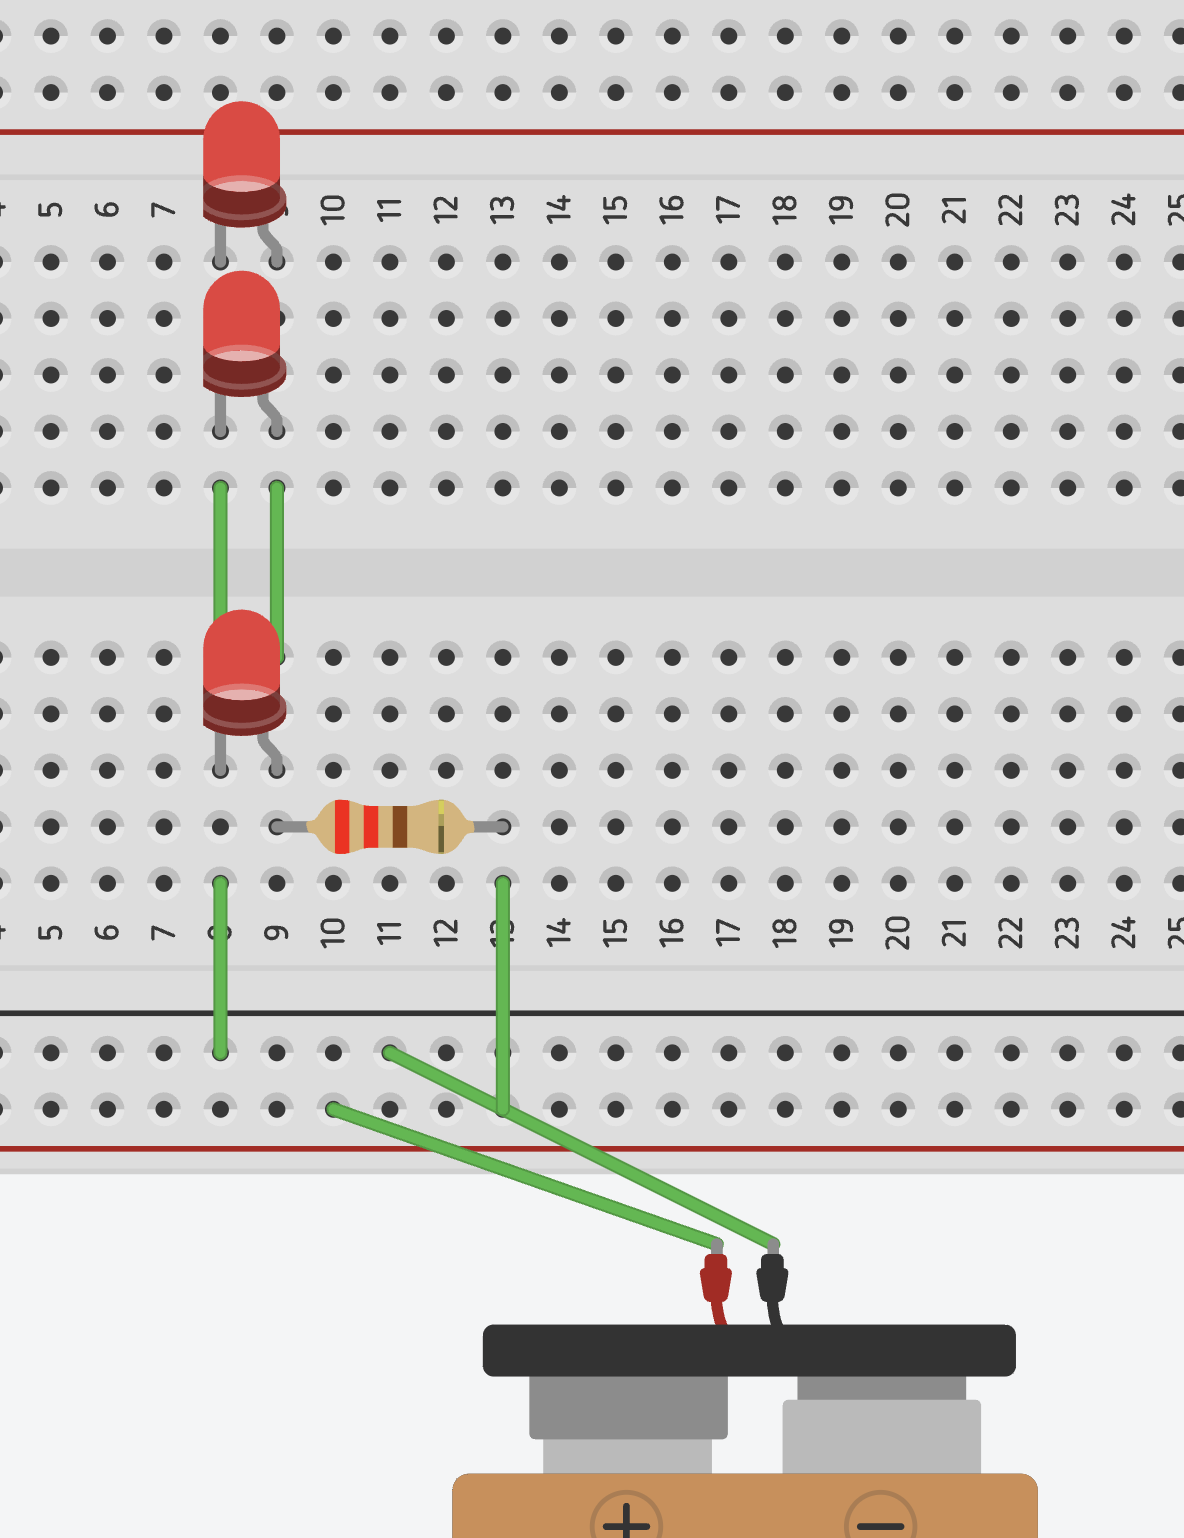
\includegraphics[width=0.5\textwidth]{led3.png}
\end{center}

With one LED, the current is \( I = (V_{\text{supply}} - V_{\text{LED}}) / R = (\SI{9}{V} - \SI{2}{V}) / \SI{470}{\ohm} \approx \SI{14.9}{mA} \). With three LEDs in parallel, the total current through R remains \SI{14.9}{mA}, but by KCL, this current divides among the three LEDs (\(\approx \SI{4.96}{mA}\) each), causing each LED's brightness to \textbf{decrease}.
\end{document}